% ------------------------------------------------------------- 
% Arquivo :  relatório modelo                                        
% ------------------------------------------------------------- 

\documentclass[brazilian,12pt,a4paper,final]{article}
% tamanhos de fontes: 10pt, 11pt ou 12pt
% opções de estilo (padrões): article, report, book, slide, letter (artigo, relatorio, livro, apresentação de slides, carta)
\usepackage[brazil]{babel}     % ifenização
%\usepackage{t1enc}            % reconhecimento dos acentos inseridos com o teclado
\usepackage[utf8]{inputenc}    %  reconhecimento dos caracteres com codificação UTF8, acentuação.
\usepackage{graphicx}          % figuras em formato eps 
%\usepackage[pdftex]{graphicx} % para produzir PDF diretamente
%\usepackage{color}             % fontes soloridas
\pdfimageresolution96
%%% fim do cabecalho %%%

%\pagestyle{empty}
\title{Análise de dados medidos em um filamento de tungstênio}
\author{Aluno: Átila Leites Romero \\ Matrícula: 144679 \\ IF-UFRGS}

\begin{document}
\maketitle

\begin{abstract}
Este trabalho apresenta uma verificação experimental da teoria de radiação de corpo negro, 
utilizando uma montagem onde foi medida a radiação emitida por uma lâmpada de tungstênio 
em função da potência elétrica fornecida.
\end{abstract}

\section{Introdução}
Segundo a lei de Stefan-Boltzmann,
$$ R_{(T)}=\sigma T^4$$
onde $R$ é a potência total irradiada, $\sigma$ é uma constante 
e $T$ é a temperatura do corpo negro. 

Mas a emissividade de corpos reais é menor que a emissividade de um corpo negro ideal.
Por isso, para corpos reais, a equação é reescrita como 
$$ R_{(T)}=\varepsilon (T)\sigma T^4$$
onde $\varepsilon$ é um número menor que $1$ e representa a emissividade do corpo.

Em outra experiência, foi verificado que as expressões
$$r=r_0+r_1(T-T_0)+r_2(T-T_0)^2$$ 
e 
$$r=r_0(\frac{T}{T_0})^\gamma$$
fornecem uma boa descrição para a
relação entre resistência e temperatura do filamento de tungstênio.

A potência total dissipada por efeito Joule pode ser calculada por 
$$P=VI$$ 
Assumindo que a energia dissipada por condução e convecção varie linearmente 
com a temperatura, pode-se afirmar que 
$$P_D=D(T-T_0)$$

Já a potência dissipada por radiação pode ser descrita pela lei de Stefan-Boltzmann, 
logo 
$$P=P_D+P_S=D(T-T_0)+S(T^4-T_0^4)$$
onde 
$$S=\sigma A 4\pi\varepsilon$$.

Como $\sigma$ é muito pequeno, 
para baixas temperaturas a dissipação por condução e convecção prevalece e,
por isso, 
$$P\simeq D(T-T_0)$$ 
e 
$$(T-T_0)\simeq \frac{P}{D}$$
o que leva a 
$$r=r_0+r_1\frac{P}{D}+r_2(\frac{P}{D})^2$$

Para altas temperaturas, a potência irradiada passa a prevalecer, 
já que cresce muito mais rápido que a potência dissipada por difusão térmica.
Neste caso,  
$$P\simeq S(T^4-T_0^4)$$ 
e, como 
$$T^4>>T_0^4$$, 
$$T^4\simeq \frac{P}{S}$$
o que leva a 
$$r=r_0\frac{1}{T_0^\gamma}(\frac{P}{S})^\frac{\gamma}{4}$$

Espera-se ainda que os dados experimentais possam ser descritos pela Lei de Planck
para radiação de corpo negro:
\[
R d\lambda=\frac{hc^2}{\lambda^5}\frac{1}{e^\frac{hc}{\lambda KT}-1} d\lambda
\]
Com a aproximação de Wien, $e^\frac{hc}{\lambda KT}-1$ é substituido 
por $e^\frac{hc}{\lambda KT}$ :
\[
R d\lambda=\frac{hc^2}{\lambda^5}e^\frac{-hc}{\lambda KT} d\lambda
\]

\section{Procedimento experimental}
Uma lâmpada de tungstênio com 20W de potência nominal foi ligada a uma fonte regulável. 
Um sensor fotoelétrico foi instalado em frente à lâmpada e ligado a um amplificador de tensão.

Foram aplicadas diferentes tensões à lâmpada.
Em cada etapa, eram medidas a corrente na lâmpada e a tensão de saída no sensor fotoelétrico, já amplificada.
Assumiu-se que a luminância detectada seria proprocional a esta tensão de saída, mesmo sendo desconhecido o valor exato desta proporção.

\section{Análise dos dados}
Para cada medida, 
a resistência da lâmpada pode ser calculada 
através da lei de Ohm: 
$$ r=V/I$$ 
onde $r$ é a resistência, $V$ a voltagem e $I$ a corrente aplicada à lâmpada. 

Para voltagens baixas, o filamento estará em baixas temperaturas,
e é esperado um comportamento polinomial entre a 
resistência elétrica do tungstênio e a potência dissipada, descritas por
$$r=r_0+r_1\frac{P}{D}+r_2(\frac{P}{D})^2$$

Os valores para $r_0$, $\frac{r_1}{D}$ e $\frac{r_2}{D^2}$
podem ser calculados
utilizando regressão polinomial.

Para voltagens mais elevadas, o filamento apresentará temperaturas elevadas, 
e é esperado um crescimento geométrico da 
potência irradiada em relação à resistência, descrito por
$$r=r_0\frac{1}{T_0^\gamma}(\frac{P}{S})^\frac{\gamma}{4}$$

Neste caso a potência dissipada é obtida a partir dos dados da luminosidade captada
pelo sensor fotoelétrico.

Rearranjando os termos para isolar as constantes, temos:
$$\frac{r}{r_0}=(\frac{1}{T_0S^\frac{1}{4}}P^\frac{1}{4})^\gamma$$

E usando logaritmos:
$$ln(\frac{r}{r_0})=\gamma[ln(\frac{1}{T_0S^\frac{1}{4}})+ln(P^\frac{1}{4})]$$
$$ln(\frac{r}{r_0})=\gamma ln(\frac{1}{T_0S^\frac{1}{4}})+\frac{\gamma}{4}ln(P)$$
$$ln(\frac{r}{r_0})=A+Bln(P)$$
onde
$$A=\gamma ln(\frac{1}{T_0S^\frac{1}{4}}); B=\frac{\gamma}{4}$$


Os valores para $\gamma ln(\frac{1}{T_0S^\frac{1}{4}})$
e $\frac{\gamma}{4}$ podem ser calculados utilizando regressão linear.

Para o valor de $r_0$ da relação $\frac{r}{r_0}$, utiliza-se o valor obtido 
nas baixas voltagens.

Utilizando logaritmos com a aproximação de Wien, espera-se que 
o gráfico de ln(L)x$\frac{1}{T}$ produza uma reta com inclinação 
$-\frac{hc}{\lambda K}$:
\[
ln(L) =C-\frac{hc}{\lambda KT}
\]

Para calcular T, usa-se:
$$T=T_0(\frac{r}{r_0})^{1/\gamma}$$

Utilizando a inclinação $\beta$ da reta, pode-se calcular a constante de Planck
através de 
\[
h=-\beta \frac{\lambda K}{c}=-\beta \dot 2.74705044 \times 10^{-19}
\]

\section{Resultados do primeiro conjunto de dados}

\begin{table}[htbp]
\centering
\begin{tabular}{|r|r|r|r|r|} 
\hline
V(V)    &       I(A)    &       L(u.a.)       &       R(Ohm)  &       P(W)    \\
\hline
0,11    &       0,12    &       5,7     &       0,92    &       0,01    \\
0,21    &       0,22    &       5,8     &       0,95    &       0,05    \\
0,30    &       0,27    &       5,9     &       1,11    &       0,08    \\
0,41    &       0,33    &       5,6     &       1,24    &       0,14    \\
0,50    &       0,35    &       6,0     &       1,43    &       0,18    \\
0,61    &       0,38    &       5,5     &       1,61    &       0,23    \\
0,70    &       0,40    &       6,0     &       1,75    &       0,28    \\
0,80    &       0,42    &       6,1     &       1,90    &       0,34    \\
0,90    &       0,44    &       5,1     &       2,05    &       0,40    \\
1,00    &       0,46    &       6,0     &       2,17    &       0,46    \\
1,10    &       0,48    &       6,0     &       2,29    &       0,53    \\
1,20    &       0,50    &       6,6     &       2,40    &       0,60    \\
1,29    &       0,52    &       6,9     &       2,48    &       0,67    \\
1,41    &       0,54    &       7,6     &       2,61    &       0,76    \\
1,50    &       0,55    &       8,7     &       2,73    &       0,83    \\
1,60    &       0,57    &       9,9     &       2,81    &       0,91    \\
1,68    &       0,59    &       11,4    &       2,85    &       0,99    \\
1,79    &       0,60    &       13,5    &       2,98    &       1,07    \\
1,88    &       0,62    &       15,7    &       3,03    &       1,17    \\
2,01    &       0,64    &       19,4    &       3,14    &       1,29    \\
2,53    &       0,72    &       44,7    &       3,51    &       1,82    \\
2,99    &       0,79    &       84,8    &       3,78    &       2,36    \\
3,46    &       0,85    &       146,2   &       4,07    &       2,94    \\
4,01    &       0,92    &       246,5   &       4,36    &       3,69    \\
4,55    &       0,98    &       370,8   &       4,64    &       4,46    \\
5,00    &       1,04    &       504     &       4,81    &       5,20    \\
5,53    &       1,09    &       689     &       5,07    &       6,03    \\
6,05    &       1,15    &       895     &       5,26    &       6,96    \\
7,02    &       1,25    &       1373    &       5,62    &       8,78    \\
8,01    &       1,34    &       1956    &       5,98    &       10,73   \\
9,00    &       1,43    &       2613    &       6,29    &       12,87   \\
10,05   &       1,52    &       3428    &       6,61    &       15,28   \\
11,02   &       1,60    &       4230    &       6,89    &       17,63   \\
12,08   &       1,69    &       5200    &       7,15    &       20,42   \\
13,04   &       1,76    &       6120    &       7,41    &       22,95   \\
 \hline
 \end{tabular}
 \caption{Primeiro conjunto de medidas.}
 \label{tabdados1}
\end{table}

No primeiro conjunto de dados, listado na tabela \ref{tabdados1}, 
não houve detecção de radiação luminosa até a voltagem de 1,1 volts.
Ou seja, até 1,1 volts, prevaleceu a difusão térmica.
Os valores calculados por regressão polinomial foram:
$$r_0=0,8148; \frac{r_1}{D}=3,820; \frac{r_2}{D^2}=-1,882$$

Na faixa de voltagens acima de 2 volts, foi notado um grande aumento da
potência dissipada, correspondente à dissipação por irradiação.

Os valores calculados por regressão linear foram:
$$\gamma ln(\frac{1}{T_0S^\frac{1}{4}}) = 1.286$$
$$\frac{\gamma}{4}=0,2963$$
$$\beta = -11284,6$$

\section{Discussão do primeiro conjunto de dados}

\begin{figure}[htbp!]
  \caption{Regressão polinomial para valores até 1,1 volts. Primeiro conjunto de medidas.}
  \label{figiniciopeq}
  \centering
    %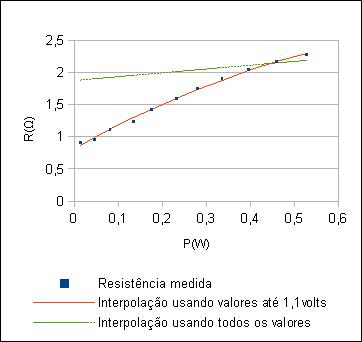
\includegraphics[scale=0.75]{iniciopeq.jpg}
    \resizebox{8.0cm}{!}{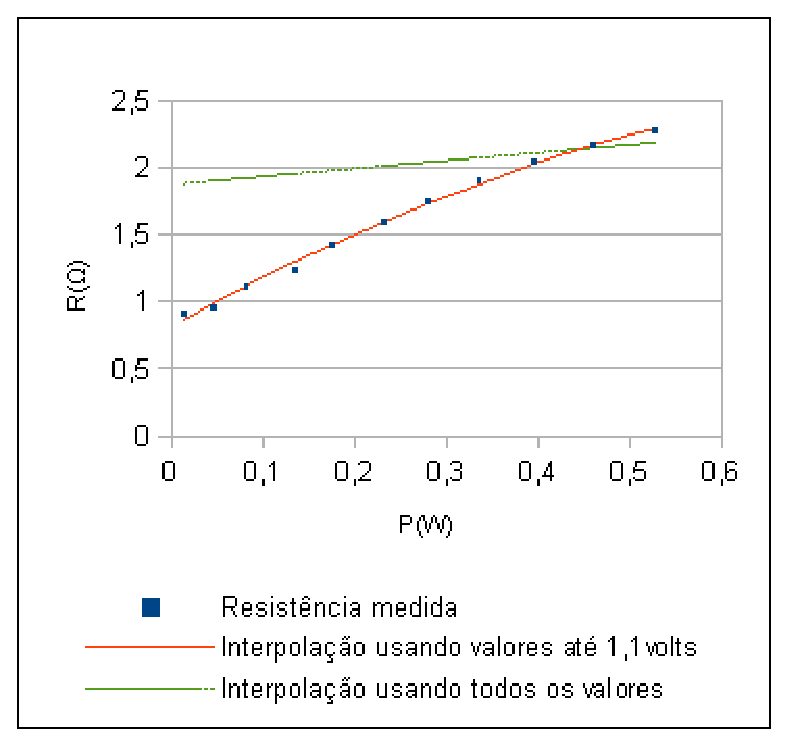
\includegraphics{iniciopeq.eps}}
\end{figure}

\begin{figure}[htbp!]
  \caption{Regressão polinomial calculada usando todas as medidas. Primeiro conjunto de medidas.}
  \label{figiniciogr}
  \centering
    %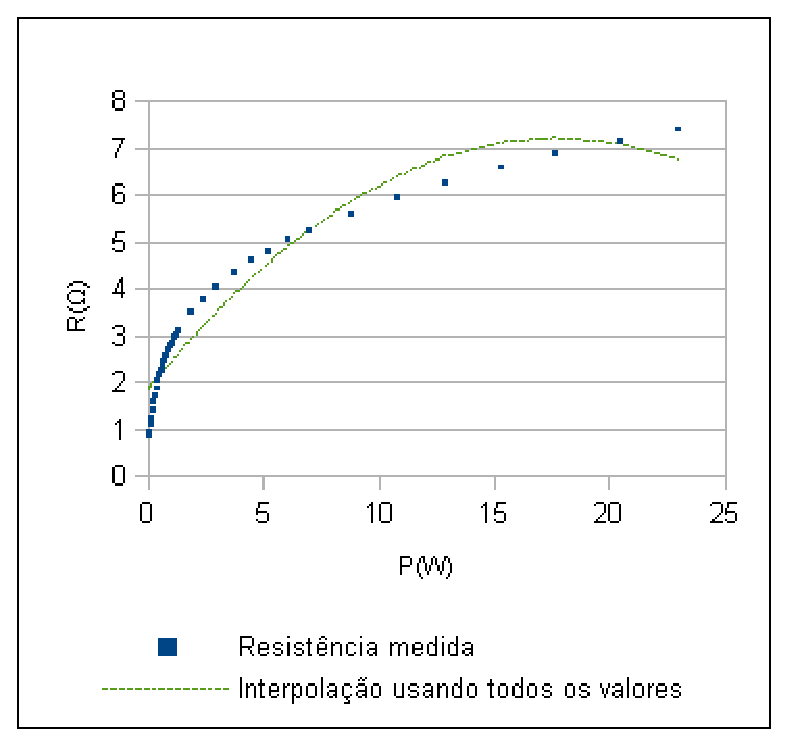
\includegraphics[scale=0.75]{iniciogr.eps}
    \resizebox{8.0cm}{!}{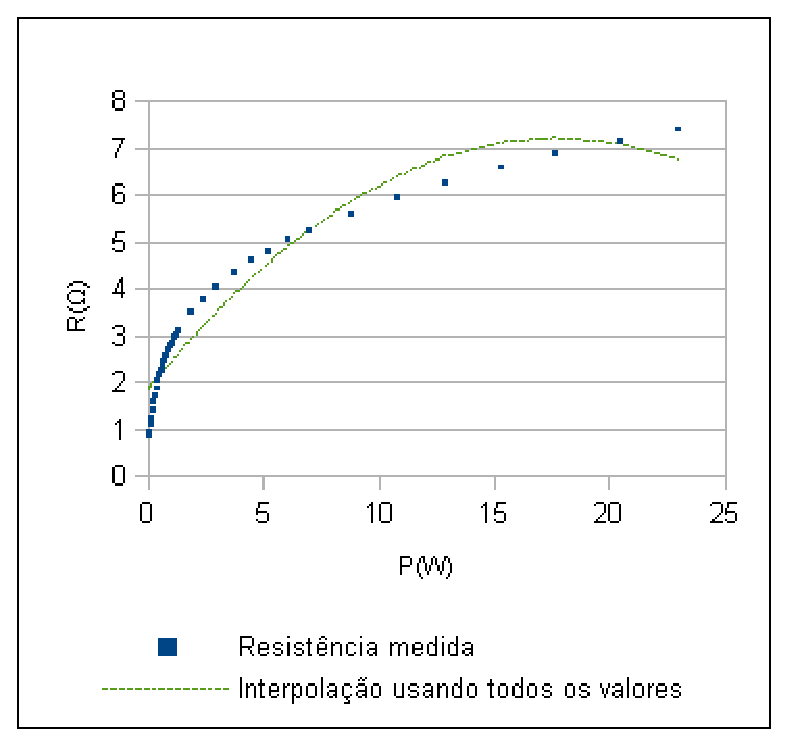
\includegraphics{iniciogr.eps}}
\end{figure}

Na figura \ref{figiniciopeq}, a regressão poninomial obtida utilizando 
valores até 1,1 volts é exibida.
Também é 
mostrado como seria o resultado nesta faixa caso todo o conjunto de dados fosse utilizado.

Na figura \ref{figiniciogr}, a regressão polinomial calculada usando o
 conjunto de dados completo é mostrada para toda a faixa de valores medidos, para
mostrar que não é uma boa aproximação.

\begin{figure}[htbp!]
  \caption{Regressão linar para os logaritmos dos valores medidos a partir de 2 volts. Primeiro conjunto de medidas.}
  \label{figfimpeq}
  \centering
    %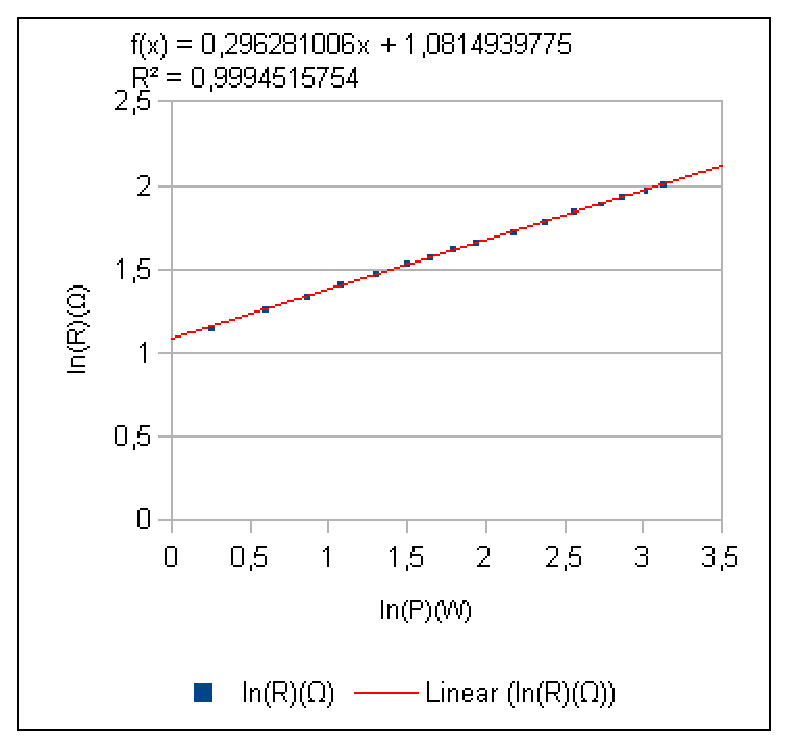
\includegraphics{fimpeq.eps}
    %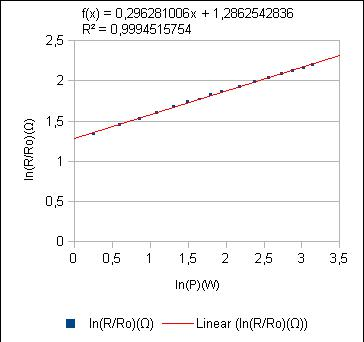
\includegraphics[scale=0.75]{fimpeq.jpg}
    \resizebox{8.0cm}{!}{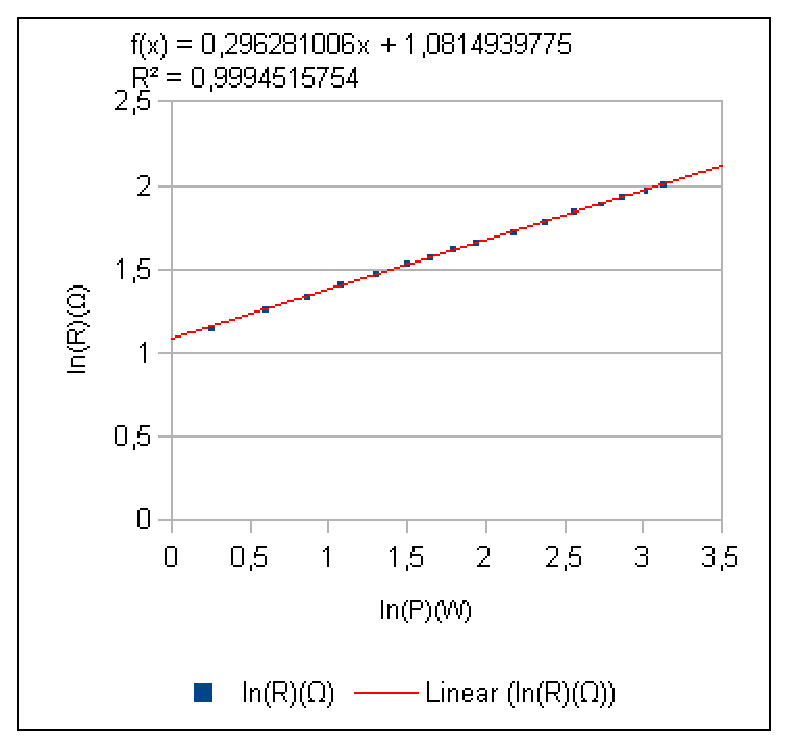
\includegraphics{fimpeq.eps}}
\end{figure}

Na figura \ref{figfimpeq}, a regressão linear obtida utilizando 
os valores medidos a partir de 2 volts é exibida.


Para mostrar que a utilização de toda a faixa de valores não fornece uma boa aproximação,
na figura \ref{figfimgr} é mostrado como ficaria a interpolação de dados se calculada desta forma.

\begin{figure}[htbp!]
  \caption{Regressão linar para os logaritmos dos valores medidos, usando toda a faixa de valores. Primeiro conjunto de medidas.}
  \label{figfimgr}
  \centering
    %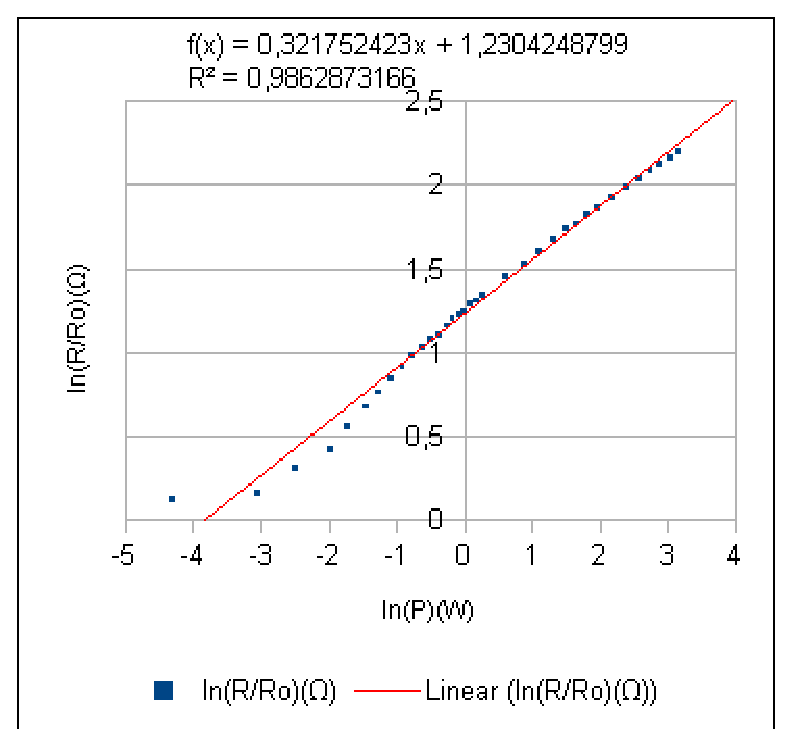
\includegraphics{fimgr.eps}
    %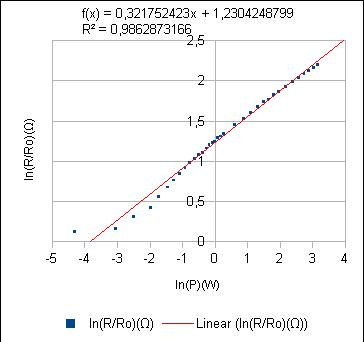
\includegraphics[scale=0.75]{fimgr.jpg}
    \resizebox{8.0cm}{!}{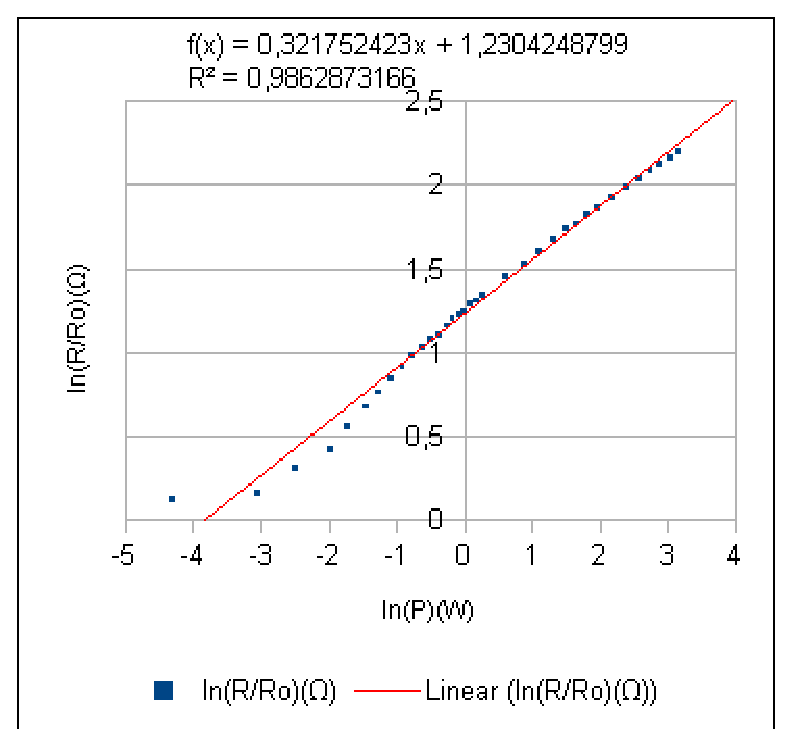
\includegraphics{fimgr.eps}}
\end{figure}

Calculando $\gamma$ temos que:
$$\gamma=4\times 0,2963=1.185$$
que é próximo ao valor $1.221$ obtido em experiência prévia,
mas o material lá utilizado pode ter características diferentes,
como densidade e impurezas, que podem explicar parte desta diferença.


\begin{figure}[htbp!]
  \caption{Regressão linear do logaritmo da luminosidade versus 1/T. Primeiro conjunto de medidas.}
  \label{fighum}
  \centering
    %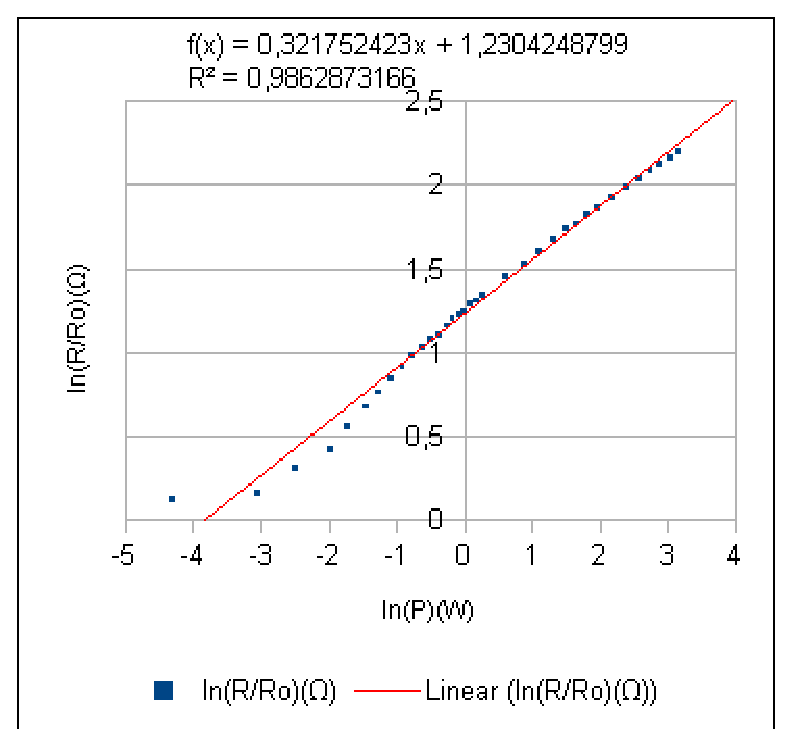
\includegraphics{fimgr.eps}
    %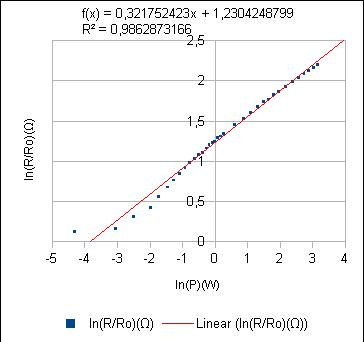
\includegraphics[scale=0.75]{fimgr.jpg}
    \resizebox{8.0cm}{!}{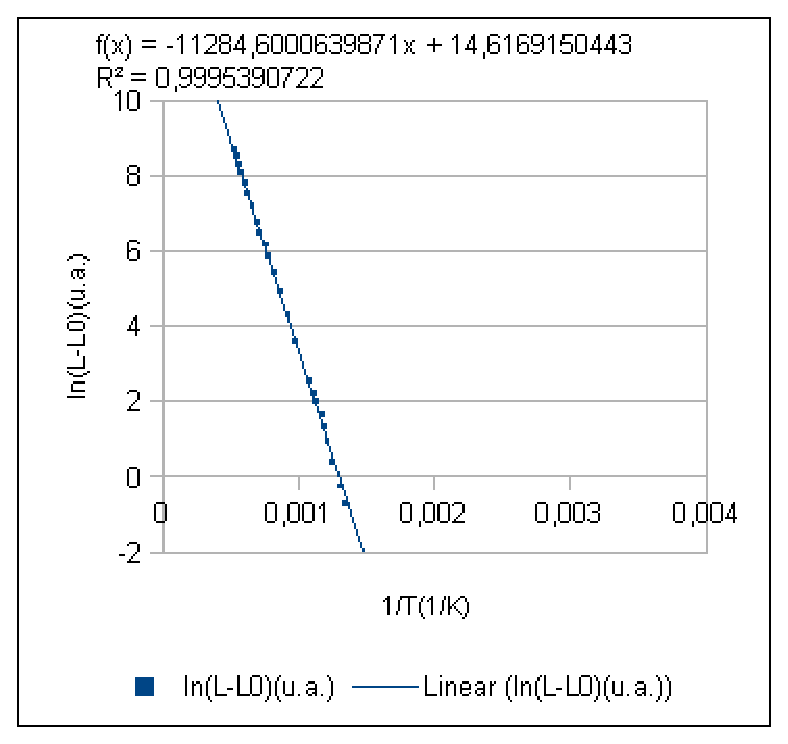
\includegraphics{h1.eps}}
\end{figure}

Na figura \ref{fighum}, foram comparados luminosidade e temperatura. A regressão linear obtida informa a inclinação $\beta$, usada para o cálculo de $h$.

O valor calculado para $h$ foi $3.09993654 \times 10^{-15} eV.s$, que apresenta
um erro de aproximadamente 25\% em relação ao valor atualmente conhecido.

É possível que um número maior de medidas em baixas voltagens fornecesse
um valor mais preciso para $r_0$, o que aumentaria a precisão do $\gamma$
calculado.

Outra fonte de erro foi a luz da sala, que estava ligada durante o 
experimento, de modo que a movimentação das pessoas pode ter influenciado
a quantidade de luz incidente no sensor, 
alterando o resultado das medidas, sobretudo nas voltagens mais baixas.

Mesmo com essas aproximações, 
foi possível observar que a potência irradiada de fato aumentou
com a quarta potência da temperatura, 
o que está de acordo com a lei de Stefan-Boltzmann.

\section{Resultados do segundo conjunto de dados}

No segundo conjunto de dados, disponíveis no Moodle, 
não houve detecção de radiação luminosa até a voltagem de 0,650 volts.
Ou seja, até 0,650 volts, prevaleceu a difusão térmica.
Os valores calculados por regressão polinomial foram:
$$r_0=0,6543; \frac{r_1}{D}=3,762; \frac{r_2}{D^2}=-1,361$$

Na faixa de voltagens acima de 2,60 volts, foi notado um grande aumento da
potência dissipada, correspondente à dissipação por irradiação.

Os valores calculados por regressão linear foram:
$$\gamma ln(\frac{1}{T_0S^\frac{1}{4}}) = 1,481$$
$$\frac{\gamma}{4}=0,3002$$

\section{Discussão do segundo conjunto de dados}

Na figura \ref{figiniciopeq2}, a regressão poninomial do segundo conjunto
de dados, obtida utilizando 
valores de até 0,650 volts é exibida.

\begin{figure}[htbp!]
  \caption{Regressão polinomial para valores até 0,650 volts. Segundo conjunto de medidas.}
  \label{figiniciopeq2}
  \centering
    %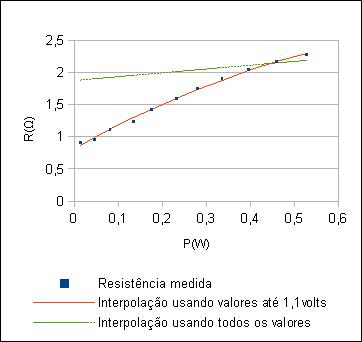
\includegraphics[scale=0.75]{iniciopeq.jpg}
    \resizebox{8.0cm}{!}{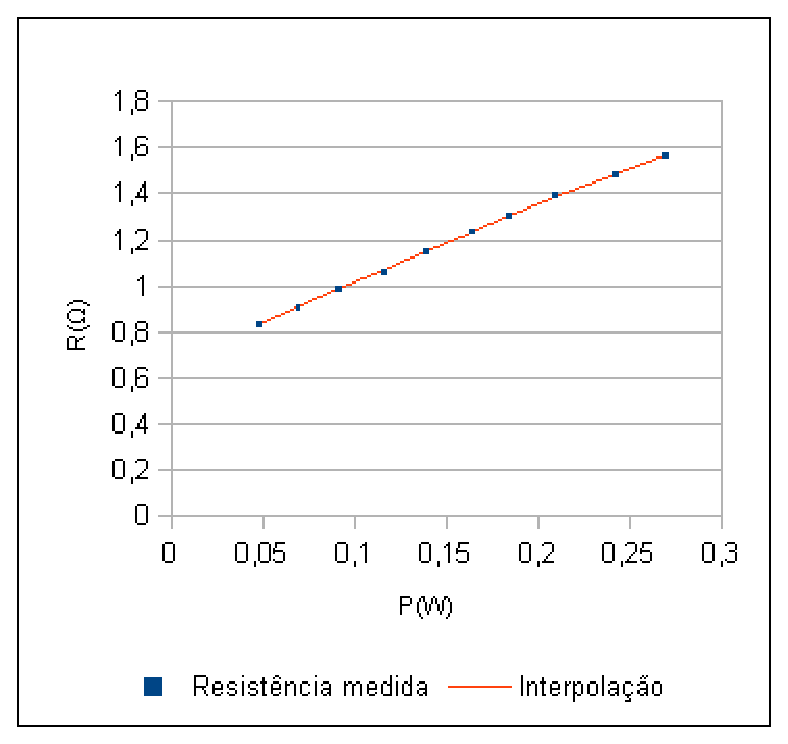
\includegraphics{iniciopeq2.eps}}
\end{figure}

Na figura \ref{figfimpeq2}, a regressão linear do segundo conjunto de dados, 
obtida utilizando os valores medidos a partir de 2,60 volts é exibida.

\begin{figure}[htbp!]
  \caption{Regressão linar para os logaritmos dos valores medidos a partir de 2,60 volts. Segundo conjunto de medidas.}
  \label{figfimpeq2}
  \centering
    %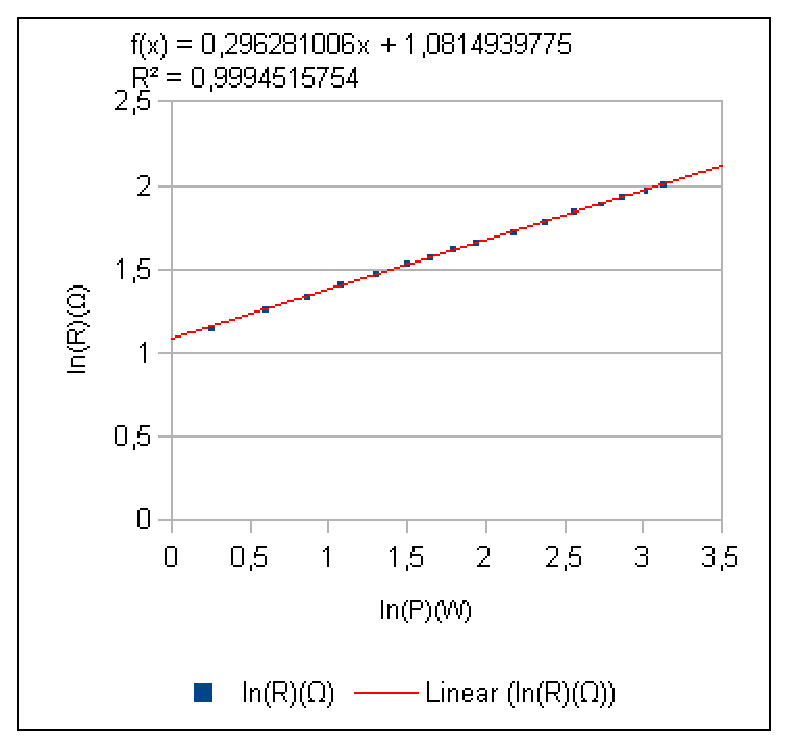
\includegraphics{fimpeq.eps}
    %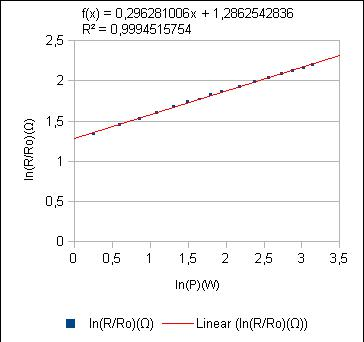
\includegraphics[scale=0.75]{fimpeq.jpg}
    \resizebox{8.0cm}{!}{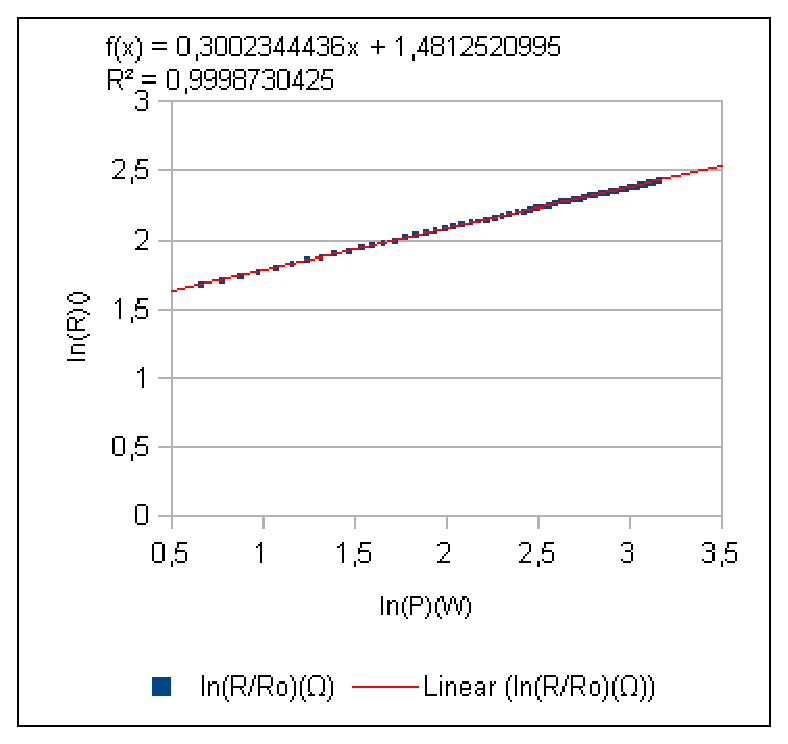
\includegraphics{fimpeq2.eps}}
\end{figure}

Isolando $\gamma$ temos que:
$$\gamma=4\times 0,3002=1,200$$
que é mais próximo ao valor $1.221$ obtido em experiência prévia que 
aquele obtido no primeiro conjunto de dados.

Na figura \ref{fighhh}, foram comparados luminosidade e temperatura. A regressão linear obtida informa a inclinação $\beta$, usada para o cálculo de $h$.

\begin{figure}[htbp!]
  \caption{Regressão linear do logaritmo da luminosidade versus 1/T. Segundo conjunto de medidas.}
  \label{fighhh}
  \centering
    %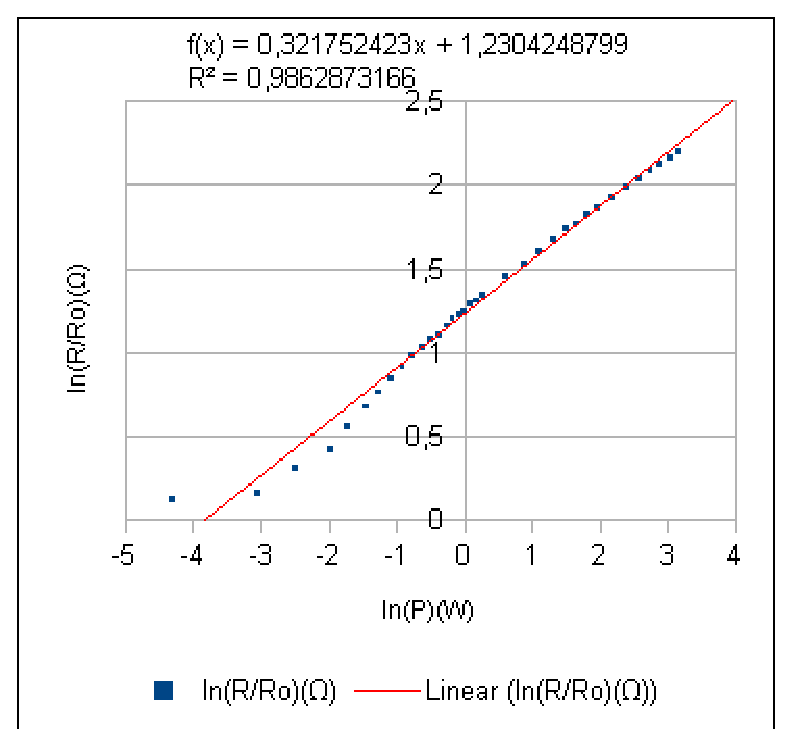
\includegraphics{fimgr.eps}
    %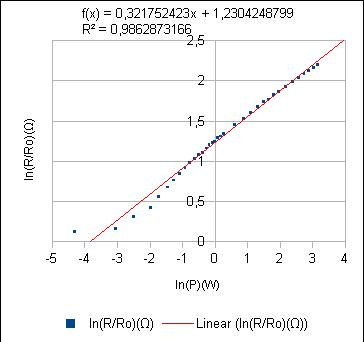
\includegraphics[scale=0.75]{fimgr.jpg}
    \resizebox{8.0cm}{!}{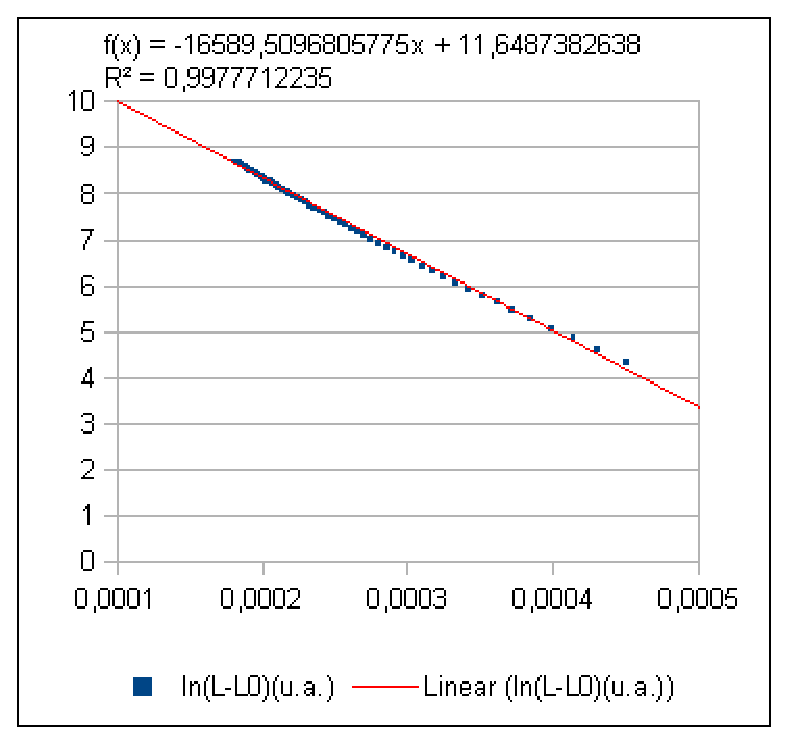
\includegraphics{h2.eps}}
\end{figure}

O valor calculado para $h$ foi $4.55721933 \times 10^{-15} eV.s$, que apresenta
um erro de aproximadamente 10\% em relação ao valor atualmente conhecido.

\section{Conclusões}
Neste experimento medimos a potência dissipada por um filamento de tungstênio
sujeito a diferentes voltagens. Foi confirmado que a difusão térmica predomina
em baixas temperaturas e que a irradiação predomina em temperaturas maiores.

O modelo de dissipação de energia para baixas temperaturas
assume que a relação entre potência dissipada e temperatura é linear
e descreveu satisfatóriamente as medidas feitas em baixa voltagem.

Para altas temperaturas, 
o modelo que considera que 
a energia dissipada é proporcional à quarta potência da temperatura 
forneceu uma descrição mais adequada para as medidas obtidas.

Os valores calculados para a constante de Planck utilizando os dois conjuntos
de dados apresentaram aproximações razoáveis em relação aos valores atualmente
conhecidos, principalemente se for considerado que a constante é um número
muito pequeno, com uma ordem de grandeza -15.

O segundo conjunto de medidas apresentou resultados melhores do que o 
primeiro, por conter mais pontos na faixa de baixas voltagens e por 
apresentar uma precisão maior, que pode ser notada pela menor variação
de luminosidade nesta mesma faixa.


%\begin{thebibliography}{99}
%\end{thebibliography}

\end{document}

